\chapter{Plano de formação}
\label{plano_de_formaçao}
\section{O nosso plano de formação}
O nosso sistema naturalmente tem como audiência pessoas que desejam um sistema informático que lhes simplifique o processo de gestão e também pessoas que não estão tão habituadas ao uso de tecnologia, portanto faz sentido que nós como "developers" forçar-nos a pensar em maneiras de ajudar o cliente a usar o nosso software. O objetivo da ePadaria nunca foi e não é fazer um software complicado de usar, logo não é necessário nenhuma formação ou "mestrado" para usar, mas devido á nossa audiência alvo temos que fazer o esforço extra só para nos certificar que o cliente consegue fazer a operação que quer.\\
Apresentamos dois métodos:\\
Oferecemos ajuda ao cliente no momento, caso for preciso responder alguma dúvida e para isso temos 2 métodos:\\
 -Contacto por e-mail;\\
 -Contacto via telefone;\\
	E possivelmente fazer a adição de um sistema de ajuda online seja automizado ou de contacto direto com o cliente.\\
O segundo método seria vídeos feitos pela equipa de desenvolvimento, como por exemplo tutoriais, que mostrassem como fazer certas operações usando a webapp com narração ( e poderiam ser animados também).\\
 \begin{figure}[H]
 	\centering
 	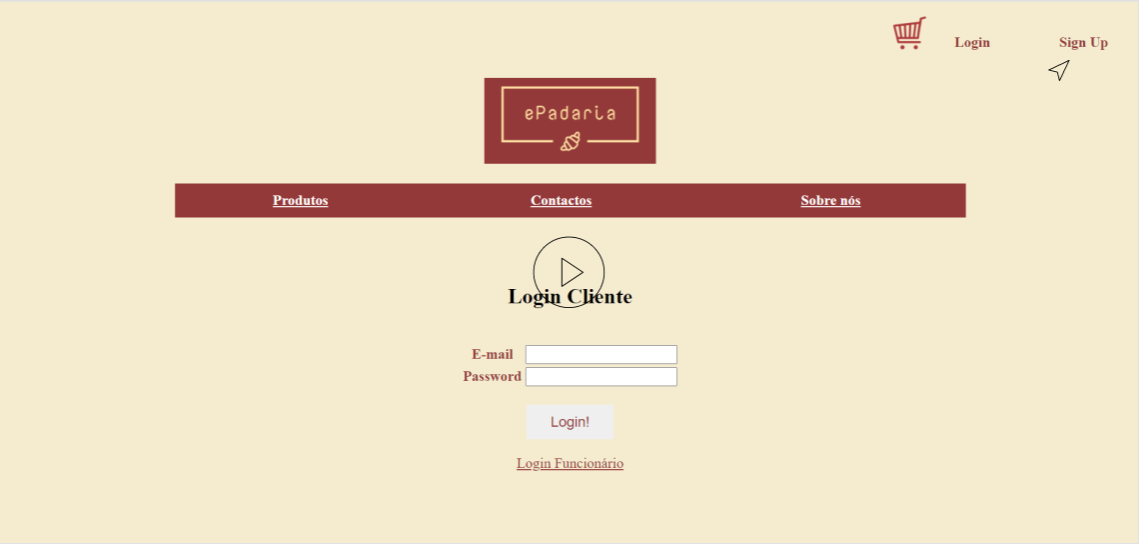
\includegraphics[width=15cm]{tutorial}
 	\caption{Exemplo de um thumbnail de um tutorial}
 	\label{fig:tutorial}
 \end{figure}